\usepackage{xcolor}
\usepackage{afterpage}
\usepackage{pifont,mdframed}
\usepackage{multicol}
\usepackage[bottom]{footmisc}


\createsection{\Grader}{Sample grader}

\renewcommand{\inputfile}{\texttt{stdin}}
\renewcommand{\outputfile}{\texttt{stdout}}
\makeatletter
\renewcommand{\this@inputfilename}{\texttt{stdin}}
\renewcommand{\this@outputfilename}{\texttt{stdout}}
\makeatother

% % % % % % % % % % % % % % % % % % % % % % % % % % % % % % % % % % % % % % % % % % %
% % % % % % % % % % % % % % % % % % % % % % % % % % % % % % % % % % % % % % % % % % %

Mojito (Monica's dog, the mascotte of OII) just finished hanging a very long
banner with the help of \emph{every other} Jack Russell Terrier living in
Matera. The banner now sits in the hall of the \emph{Pentasuglia High-School},
where the awards ceremony of the OII will soon take place. Once finished with
the banner, Mojito noticed that the long list of sponsor sometimes contains
\textbf{pangrams}: sentences that use every letter of the alphabet.

\begin{figure}[H]
  \centering
  \frame{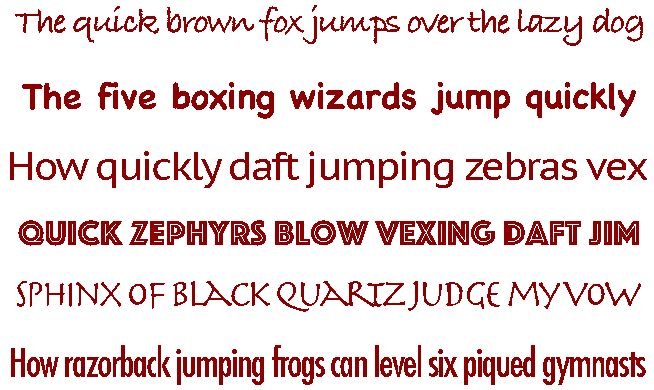
\includegraphics{pangram.pdf}}
  \caption{A selection of six different pangrams\footnotemark}
\end{figure}
\footnotetext{Pangrams are not just Mojito's past time fun, they're actually
useful in the real world. For example, pangrams are used in typography to test
how different fonts render on print. Moreover, encoding a pangram is a good way
to test your knowledge of Morse code. In the 80s, the Italian writer Umberto Eco
was obsessed with pangrams. He found a perfect one that uses all $21$ letters of
the Italian alphabet:\\\phantom{xxxxxxxxxxxxxxxxxxxxxxxxxxxxxxxxxxxxx}\emph{``Tv?
Quiz, BR, FLM, DC... Oh, spenga!''}}

Clearly, finding long pangrams is quite easy. What's hard is to find short ones.
The absolute shortest pangrams are also called \textbf{perfect pangrams}: they
use each letter \emph{exactly once}:%
%
\begin{center}
  \texttt{Mr Jock TV quiz PhD bags few lynx}
\end{center}%
%
Sadly, it's not guaranteed that a perfect pangram will appear in the banner.
When this happens, Mojito will settle for \textbf{minimal pangrams} (i.e.
pangrams with the lowest possible length) in the banner.

Feeling inspired from this discovery, Mojito decided to organize a game to play
with his helpers: each of the $\mathbf{46\,337}$ Jack Russell Terriers will have
to show the others a minimal pangram from the banner. To do that, the dogs must
highlight each alphabet letter in the banner in a different way than what all
the other dogs did previously. Before starting this challenge, Mojito wants to
know how many distinct ways there are to perform this ``highlighting''... he
really doesn't want to lose!

More precisely, the banner contains a string $V$ of $N$ characters, each
character belonging to an alphabet of $K$ symbols.\footnote{The banner contains
letters but also: numbers, special characters, emojis, the batman symbol, \dots}
The symbols are represented with integers from $0$ to $K-1$. A
\emph{highlighting} maps each symbol $j$ of the alphabet to a position $x_j$ of
the string $V$ where the symbol appears, i.e. such that $V[x_j] = j$. Two
highlightings are different if they map different positions $x_j \neq x'_j$ to
at least one symbol $j$, even if they correspond to the same pangram. A
highlighting is \emph{minimal} if it encloses a minimal pangram (i.e. if the
maximum difference $x_j - x_i$ between the positions of two occurrences is the
minimum possible). Mojito wants to count how many minimal highlightings exist,
\textbf{modulo} $\mathbf{46\,337}$: help him!

% % % % % % % % % % % % % % % % % % % % % % % % % % % % % % % % % % % % % % % % % % %
% % % % % % % % % % % % % % % % % % % % % % % % % % % % % % % % % % % % % % % % % % %


\Implementation

\begin{danger}
  It's crucial to perform the modulo operation after each addition because the
  intermediate values generated might require more than 32 bit to be stored.
  When looking for some result modulo $M$, we suggest exploting the fact that
  ($A$ + $B$ + $C$) modulo $M$ = ((($A$ + $B$) modulo $M$) + $C$) modulo $M$.
  The same thing is true for the multiplication. In this way, the intermediate
  results are always kept modulo $M$ and can be stored in a normal integer
  variable.
\end{danger}

You should submit a single file, with either a \texttt{.c} or \texttt{.cpp}
extension.

\begin{warning}
Among the attachments in this task you will find a template \texttt{pangramma.c}
or \texttt{pangramma.cpp} with a sample implementation.
\end{warning}

You will have to implement the following function:

\begin{center}\begin{tabularx}{\textwidth}{|c|X|}
\hline
C    & \verb|int conta(int N, int K, int* V);|\\
C++  & \verb|int conta(int N, int K, vector<int>& V);|\\
\hline
\end{tabularx}\end{center}

\begin{itemize}[nolistsep]
  \item The integer $N$ is the length of array \texttt{V}, i.e. the total number
        of letters in the banner.
  \item The integer $K$ is the number of different symbols in the alphabet.
  \item The array \texttt{V}, indexed from $0$ to $N-1$, specifies the symbol
        contained in each position.
  \item The function should return the number of differet minimal highlightings
        modulo $46\,337$.
\end{itemize}

\medskip

The grader will call the \texttt{conta} function and will print the returned
value in the output file.

% % % % % % % % % % % % % % % % % % % % % % % % % % % % % % % % % % % % % % % % % % %
% % % % % % % % % % % % % % % % % % % % % % % % % % % % % % % % % % % % % % % % % % %


\Grader

Among this task's attachments you will find a simplified version of the grader
used during evaluation, which you can use to test your solutions locally. The
sample grader reads data from \inputfile{}, calls the functions that you should
implement and writes back on \outputfile{} using the following format.

The input file is formed by $2$ lines:
\begin{itemize}[nolistsep,itemsep=2mm]
\item Line $1$: two integers $N$ and $K$.
\item Line $2$: $N$ integers \texttt{V[$i$]} for $i = 0\ldots N-1$.
\end{itemize}

The output file is formed by a single line which contains the value returned by
the \texttt{conta} function.

% % % % % % % % % % % % % % % % % % % % % % % % % % % % % % % % % % % % % % % % % % %
% % % % % % % % % % % % % % % % % % % % % % % % % % % % % % % % % % % % % % % % % % %


\Constraints

\begin{itemize}[nolistsep, itemsep=2mm]
    \item $1 \le K \le N \le 1\,000\,000$.
    \item $0 \le$ \texttt{V[$i$]} $\le K-1$ for $i = 0\dots N-1$.
    \item Every symbol appears at least once in the string.
\end{itemize}

% % % % % % % % % % % % % % % % % % % % % % % % % % % % % % % % % % % % % % % % % % %
% % % % % % % % % % % % % % % % % % % % % % % % % % % % % % % % % % % % % % % % % % %


\Scoring

Your program will be tested on a number of testcases grouped in subtasks. In
order to obtain the score associated to a subtask, you need to correctly solve
all testcases of which it is formed.

\begin{itemize}[nolistsep,itemsep=2mm]
  \item \textbf{\makebox[2.3cm][l]{Subtask \phantom{1}1} [\phantom{1}0 points]}: Sample testcases.
  \item \textbf{\makebox[2.3cm][l]{Subtask \phantom{1}2} [\phantom{1}5 points]}: $K = 2$.
  \item \textbf{\makebox[2.3cm][l]{Subtask \phantom{1}3} [\phantom{1}7 points]}: $N \le 30$.
  \item \textbf{\makebox[2.3cm][l]{Subtask \phantom{1}4} [14           points]}: $N \le 300$.
  \item \textbf{\makebox[2.3cm][l]{Subtask \phantom{1}5} [13           points]}: $N \le 5000$.
  \item \textbf{\makebox[2.3cm][l]{Subtask \phantom{1}6} [12           points]}: There is at least one \textit{perfect pangram} in the banner.
  \item \textbf{\makebox[2.3cm][l]{Subtask \phantom{1}7} [11           points]}: The minimal pangram has a length of at most $60$.
  \item \textbf{\makebox[2.3cm][l]{Subtask \phantom{1}8} [10           points]}: The number of minimal highlightings is at most $10^9$.
  \item \textbf{\makebox[2.3cm][l]{Subtask \phantom{1}9} [\phantom{1}9 points]}: $N \le 500\,000$.
  \item \textbf{\makebox[2.3cm][l]{Subtask           10} [10           points]}: No limits.
  \item \textbf{\makebox[2.3cm][l]{Subtask           11} [\phantom{1}7 points]}: \raisebox{0.05cm}{{\fontencoding{U}\fontfamily{futs}\selectfont\char 66\relax}}\emph{Special case:} $1\,000\,000 \le K \le N \le 5\,000\,000$.
  \item \textbf{\makebox[2.3cm][l]{Subtask           12} [\phantom{1}2 points]}: \raisebox{0.05cm}{{\fontencoding{U}\fontfamily{futs}\selectfont\char 66\relax}}\emph{Special case:} $5\,000\,000 \le K \le N \le 9\,000\,000$.
\end{itemize}

% % % % % % % % % % % % % % % % % % % % % % % % % % % % % % % % % % % % % % % % % % %
% % % % % % % % % % % % % % % % % % % % % % % % % % % % % % % % % % % % % % % % % % %


\Examples

\begin{example}
\exmpfile{pangramma.input0.txt}{pangramma.output0.txt}%
\exmpfile{pangramma.input1.txt}{pangramma.output1.txt}%
\exmpfile{pangramma.input2.txt}{pangramma.output2.txt}%
\exmpfile{pangramma.input3.txt}{pangramma.output3.txt}%
\end{example}

% % % % % % % % % % % % % % % % % % % % % % % % % % % % % % % % % % % % % % % % % % %
% % % % % % % % % % % % % % % % % % % % % % % % % % % % % % % % % % % % % % % % % % %


\Explanation

In the \textbf{first sample testcase} there are two minimal pangrams, which happen to also be perfect:%
\begin{center}
  \tt
  \begin{tikzpicture}
    \node[draw,dashed] at (-0.95, 0) {\colorbox{yellow!90}{2},\colorbox{yellow!90}{0},\colorbox{yellow!90}{1}};
    \node[text] at (0.95, -0.03) {, 1, 2, 0};
  \end{tikzpicture}
  
  \begin{tikzpicture}
    \node[text] at (-0.92, -0.03) {2, 0, 1,};
    \node[draw,dashed] at (0.92, 0) {\colorbox{yellow!90}{1},\colorbox{yellow!90}{2},\colorbox{yellow!90}{0}};
  \end{tikzpicture}
\end{center}

There are longer pangrams, but they should not be counted:%
\begin{center}
  \tt
  \begin{tikzpicture}
    \node[text] at (-1.51, 0) {2,};
    \node[draw,dashed] at (0, 0) {0, 1, 1, 2};
    \node[text] at (1.51, 0) {, 0};
  \end{tikzpicture}
\end{center}
In total, there are $\mathbf{2}$ different ways to highlight a minimal pangram.

In the \textbf{second sample testcase} there are again two minimal pangrams, but they are not perfect pangrams. There are $\mathbf{4}$ minimal highlightings:%
\begin{center}
  \tt
  \begin{tikzpicture}
    \node[draw,dashed] at (-1.2, 0) {\colorbox{yellow!90}{0},\,\colorbox{yellow!90}{1}, 1,\,\colorbox{yellow!90}{2}};
    \node[text] at (1.1, -0.03) {, 1, 1, 0};
  \end{tikzpicture}
  \quad
  \begin{tikzpicture}
    \node[text] at (-1.1, -0.03) {0, 1, 1, };
    \node[draw,dashed] at (1.1, 0) {\colorbox{yellow!90}{2},\,\colorbox{yellow!90}{1}, 1,\,\colorbox{yellow!90}{0}};
  \end{tikzpicture}

  \begin{tikzpicture}
    \node[draw,dashed] at (-1.2, 0) {\colorbox{yellow!90}{0}, 1,\,\colorbox{yellow!90}{1},\,\colorbox{yellow!90}{2}};
    \node[text] at (1.1, -0.03) {, 1, 1, 0};
  \end{tikzpicture}
  \quad
  \begin{tikzpicture}
    \node[text] at (-1.1, -0.03) {0, 1, 1, };
    \node[draw,dashed] at (1.1, 0) {\colorbox{yellow!90}{2}, 1,\,\colorbox{yellow!90}{1},\,\colorbox{yellow!90}{0}};
  \end{tikzpicture}
\end{center}

In the \textbf{third sample testcase} there is only one perfect pangram, in the
middle, so there is only one minimal highlighting.

In the \textbf{fourth sample testcase} there are $2$ minimal pangrams,
respectively with $6$ and $4$ minimal highlightings, for a total of $10$.
